\section{Sentiment Analysis}
\label{sec:sentiment}
We apply classification techniques on a sample dataset taken from YouTube. The dataset can be downloaded from~\cite{youtubedata}. 
It includes $691407$ comments for $200$ most trending YouTube videos in US in a two weeks period. The same source also offers a similar dataset for the most trending videos in GB. We will use a fraction of this dataset as development set. The data contains video title, channel title, category, tags, number of views, likes and dislikes and user reviews. In this section, we first explain our methodology to classify comments into three categories, positive, neutral and negative. Then, we apply a number of classification methods on the data and compare their performance with each other. 

\begin{figure}%
\centering
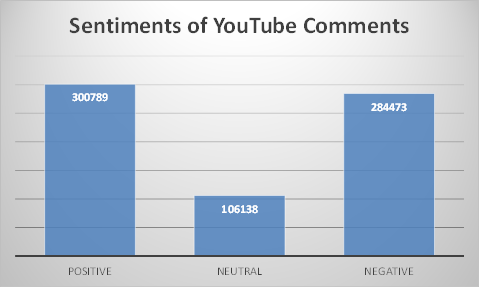
\includegraphics[width=0.6\columnwidth]{figures/datastats.png}%
\caption{YouTube Dataset Statistics}%
\label{fig:datastats}%
\end{figure}

\subsection{Label Generation}
\label{sec:label}
Our goal is to apply classification techniques on the YouTube data in order to understand whether a new comment bears positive or negative sentiment. However, there are no labels classifying the comments based on their sentiment. Considering the large number of comments, it was not possible for us to manually label a reasonable fraction of this dataset. Consequently, we used TextBlob~\cite{textblob} library for Python to generate the labels. TextBlob applies Natural language Processing techniques to estimate the \textbf{polarity} of each comment independently from the rest of the comments, and only based on its content. For us, it replaces the burdensome task of manual labeling. TextBlob generates polarity scores in the range of $(-1,1)$. We convert them into categorical data using Equation~\ref{eq:sentiment}. Statistics on the size of each class is shown in Figure~\ref{fig:datastats}.
\begin{eqnarray}
\textrm{sentiment}=
\begin{cases}
-1 & \textrm{polarity} < 0\\
0 & \textrm{polarity} = 0\\
1 & \textrm{polarity} > 0
\end{cases}
\label{eq:sentiment}
\end{eqnarray}
Words that happen more frequently in positive and negative comments are shown as word clouds in Figures~\ref{fig:poscloud} and~\ref{fig:negcloud}.

\begin{figure}[h]
\centering
\begin{minipage}{0.49\textwidth}
\centering
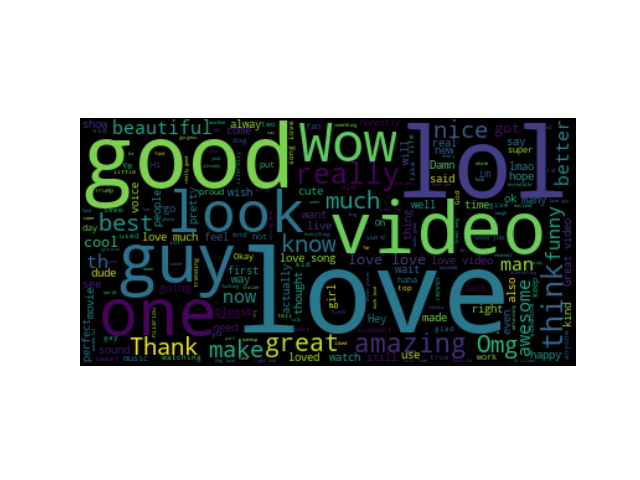
\includegraphics[width=1.0\linewidth]{figures/pos_WordCloud.png}
\caption{Word cloud for positive comments.}
\label{fig:poscloud}
\end{minipage}
\begin{minipage}{0.49\textwidth}
\centering
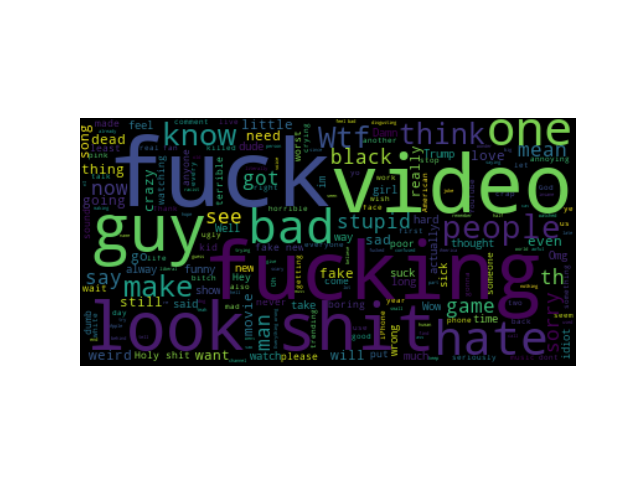
\includegraphics[width=1.0\linewidth]{figures/neg_WordCloud.png}
\caption{Word cloud for negative comments.}
\label{fig:negcloud}
\end{minipage}
\end{figure}

\subsection{Feature Extraction}
\label{sec:feature}
We use TF-IDF to convert comments into feature vectors. In this technique, stop words are first removed and the remaining words are stemmed. Stop words are commonly used words such as \textit{the} which are filtered out before the analysis. Stemming is the process of reducing derived words to their common root known as stem. For instance, \textit{going} and \textit{goes} both come from the stem \textit{go}. TF (Term Frequency) counts the number of times a word has occurred in each document. However, the number of occurrences of words is in general higher for longer documents. Then, it is helpful to divide the number of word occurrences by the number of words in the document. The output of TF is a sparse matrix mapping documents to a normalized vector representing how many times each word has occurred in them. IDF (Inverse Document Frequency) accounts for the number of occurrences of a word in the entire corpus. Namely, some words are more likely than others to happen in a given corpus of documents. Then, we scale TF terms by a decreasing function of the number of occurrences of each word in the whole corpus which is indeed the IDF term.

\subsection{Experiments and Evaluation}
\label{sec:experiments}
In order to measure the performance of different classification techniques on the YouTube data, we split the data from US comments into train and test subsets. To generate the train set, we randomly choose $80\%$ of the comments from each of the three categories. The remaining comments form the test set. We use $20\%$ of the GB comments as development set. 
We ran three different classification techniques on the data, including Ridge Classifier, Bernoulli Naive Bayes and SVM. Table~\ref{tab:accuracy} shows the accuracy measured on test and dev sets. Naive Bayes classifier has the worst performance among all methods. This result is predictable as the conditional independence condition required by the Naive Bayes classifier is not satisfied in this dataset. In particular, the probability of two words happening in a comment given the category of the comment are not independent from one another. On this dataset, Ridge classifer has the best performance.

\begin{table}%
\centering
\begin{tabular}{|l|c|r|}
\hline
Model & Test Error & Dev Error \\
\hline
Ridge Classifier & $0.914$ & $0.905$ \\
\hline
Bernoulli NB & $0.709$ & $0.715$ \\
\hline
LinearSVC & $0.956$ & $0.951$ \\
\hline
\end{tabular}
\caption{Accuracy of different classification techniques on YouTube comments.}
\label{tab:accuracy}
\end{table}